\section{Fall 4: Box}
\label{sec:testcase-box}\ohead{Sebastian Schmitt}
Im vierten Testfall wird versucht eine Box anhand von fünf Bildern zu rekonstruieren.
Diese ist in \autoref{fig:box-image} zu sehen.

Die \autoref{tab:box-results} zeigt die Ergebnisse der Rekonstruktion.
Es fällt auf, dass nur vergleichsweise sehr wenige Matches gefunden werden.
Betracht man jedoch in \autoref{fig:box-first-pair-with-matches} wo Keypoints und Matches liegen, erkennt man, dass die meisten Matches durchaus direkt an der Box bzw. an dem Kissen auf der Box gefunden wurden.
Besonders das Kissen und die Vorderseite der Box kann man in \autoref{fig:box-model} gut erkennen.
Diese guten Matches kommen zustande, da es in den Bildern klare Flächen mit identifizierbaren Kanten gibt.
Dass auf der Seite der Box keine Matches gefunden wurden, ist dadurch zu erklären, dass jeweils nur ein Bild existiert auf welchem eine Boxseite zu erkennen ist.
Betrachtet man \autoref{fig:box-model-2}, so erkennt man etwas oberhalb deutlich weitere Punkte zu Kissen bzw. Boxdeckel, welche eigentlich tiefer liegen müssten.
Dies lässt ähnlich wie in \autoref{sec:textcase-chair} eine ungenaue Skalierung des Translationsvektors vermuten.

\begin{figure}
    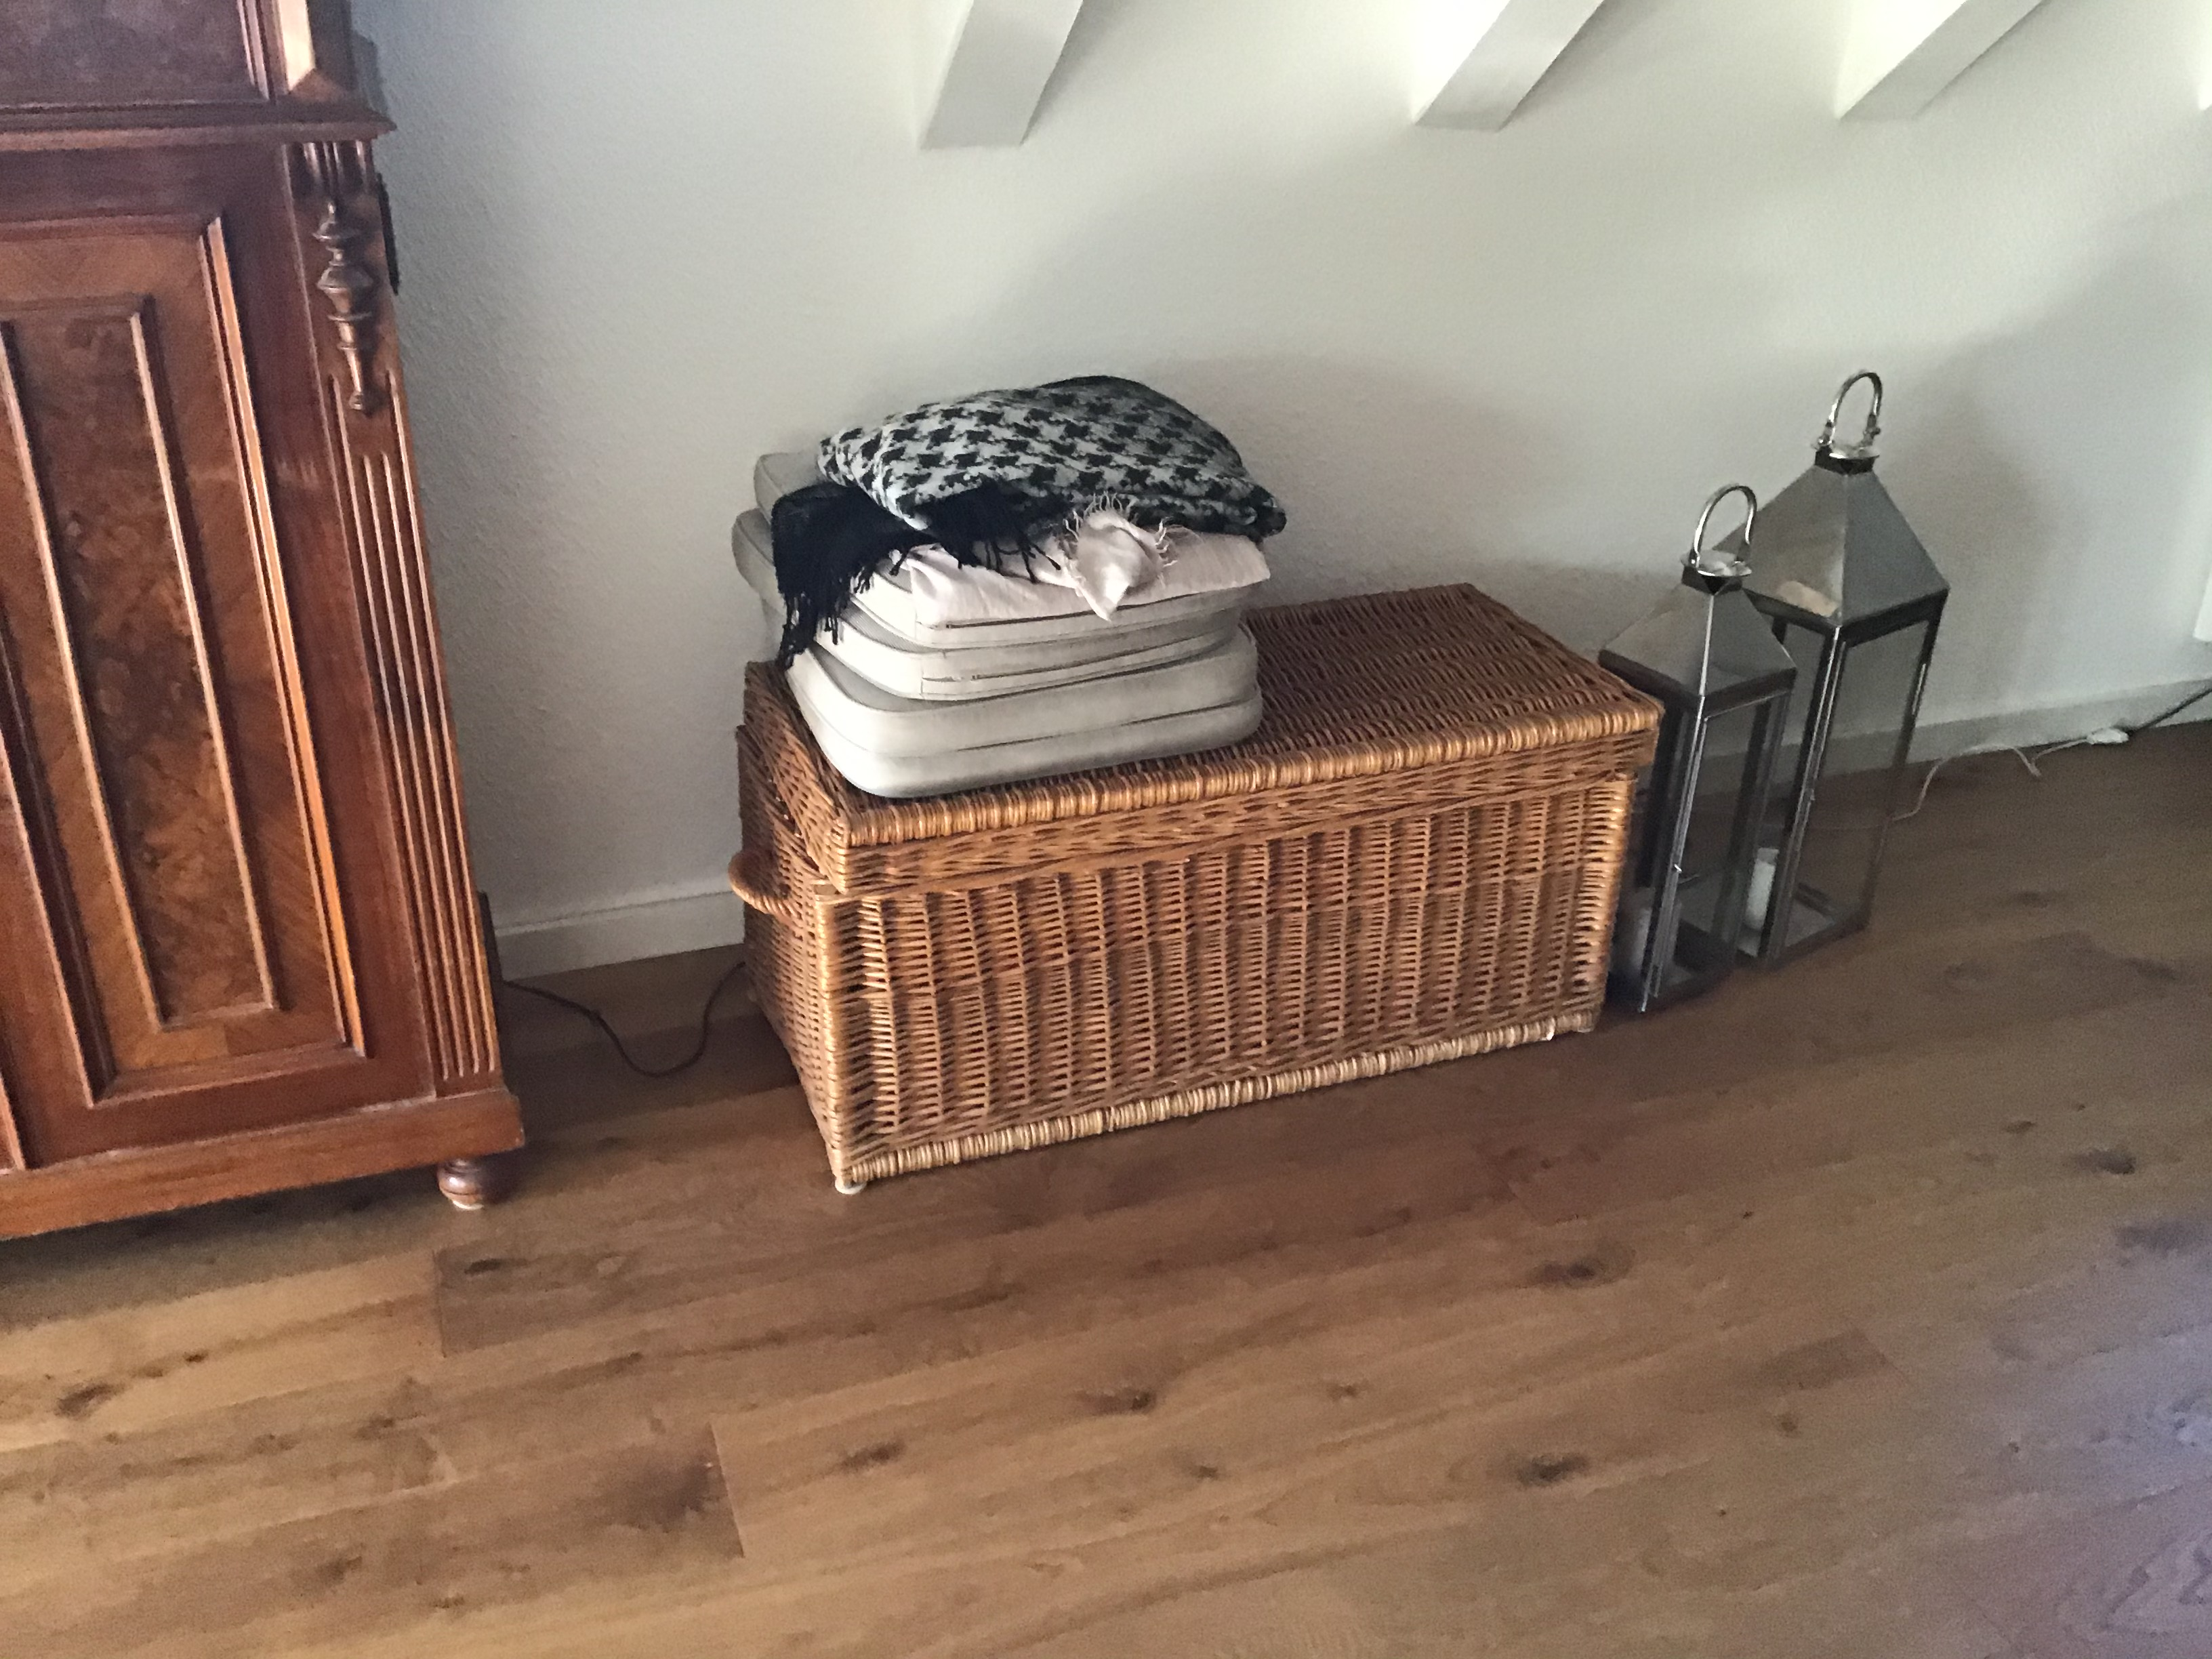
\includegraphics[width=\textwidth]{src/img/box.jpg}
    \caption{Die Box welche rekonstruiert wird}
    \label{fig:box-image}
\end{figure}

\begin{table}
    \begin{tabularx}{\textwidth}{cXXXX}
        \toprule
        Bildpaar & Anzahl der Matches & Anzahl der Weltpunkte & Anzahl der Weltpunkte für Skalierung & angewandte Skalierung \\ 
        \midrule
        1 & \makecell[r]{267} & \makecell[r]{215} & \makecell[r]{-} & \makecell[r]{-} \\
        2 & \makecell[r]{914} & \makecell[r]{215} & \makecell[r]{81} & \makecell[r]{0,667182} \\
        3 & \makecell[r]{433} & \makecell[r]{359} & \makecell[r]{117} & \makecell[r]{1,34628} \\
        4 & \makecell[r]{1.170} & \makecell[r]{1.154} & \makecell[r]{131} & \makecell[r]{0,542451} \\
        \midrule
        Summe & \makecell[r]{2.786} & \makecell[r]{2.542} & \makecell[r]{329} & \makecell[r]{-} \\
        \bottomrule
    \end{tabularx}
    \caption{Ergebnis der Rekonstruktion der Box}
    \label{tab:box-results}
\end{table}

\begin{figure}
    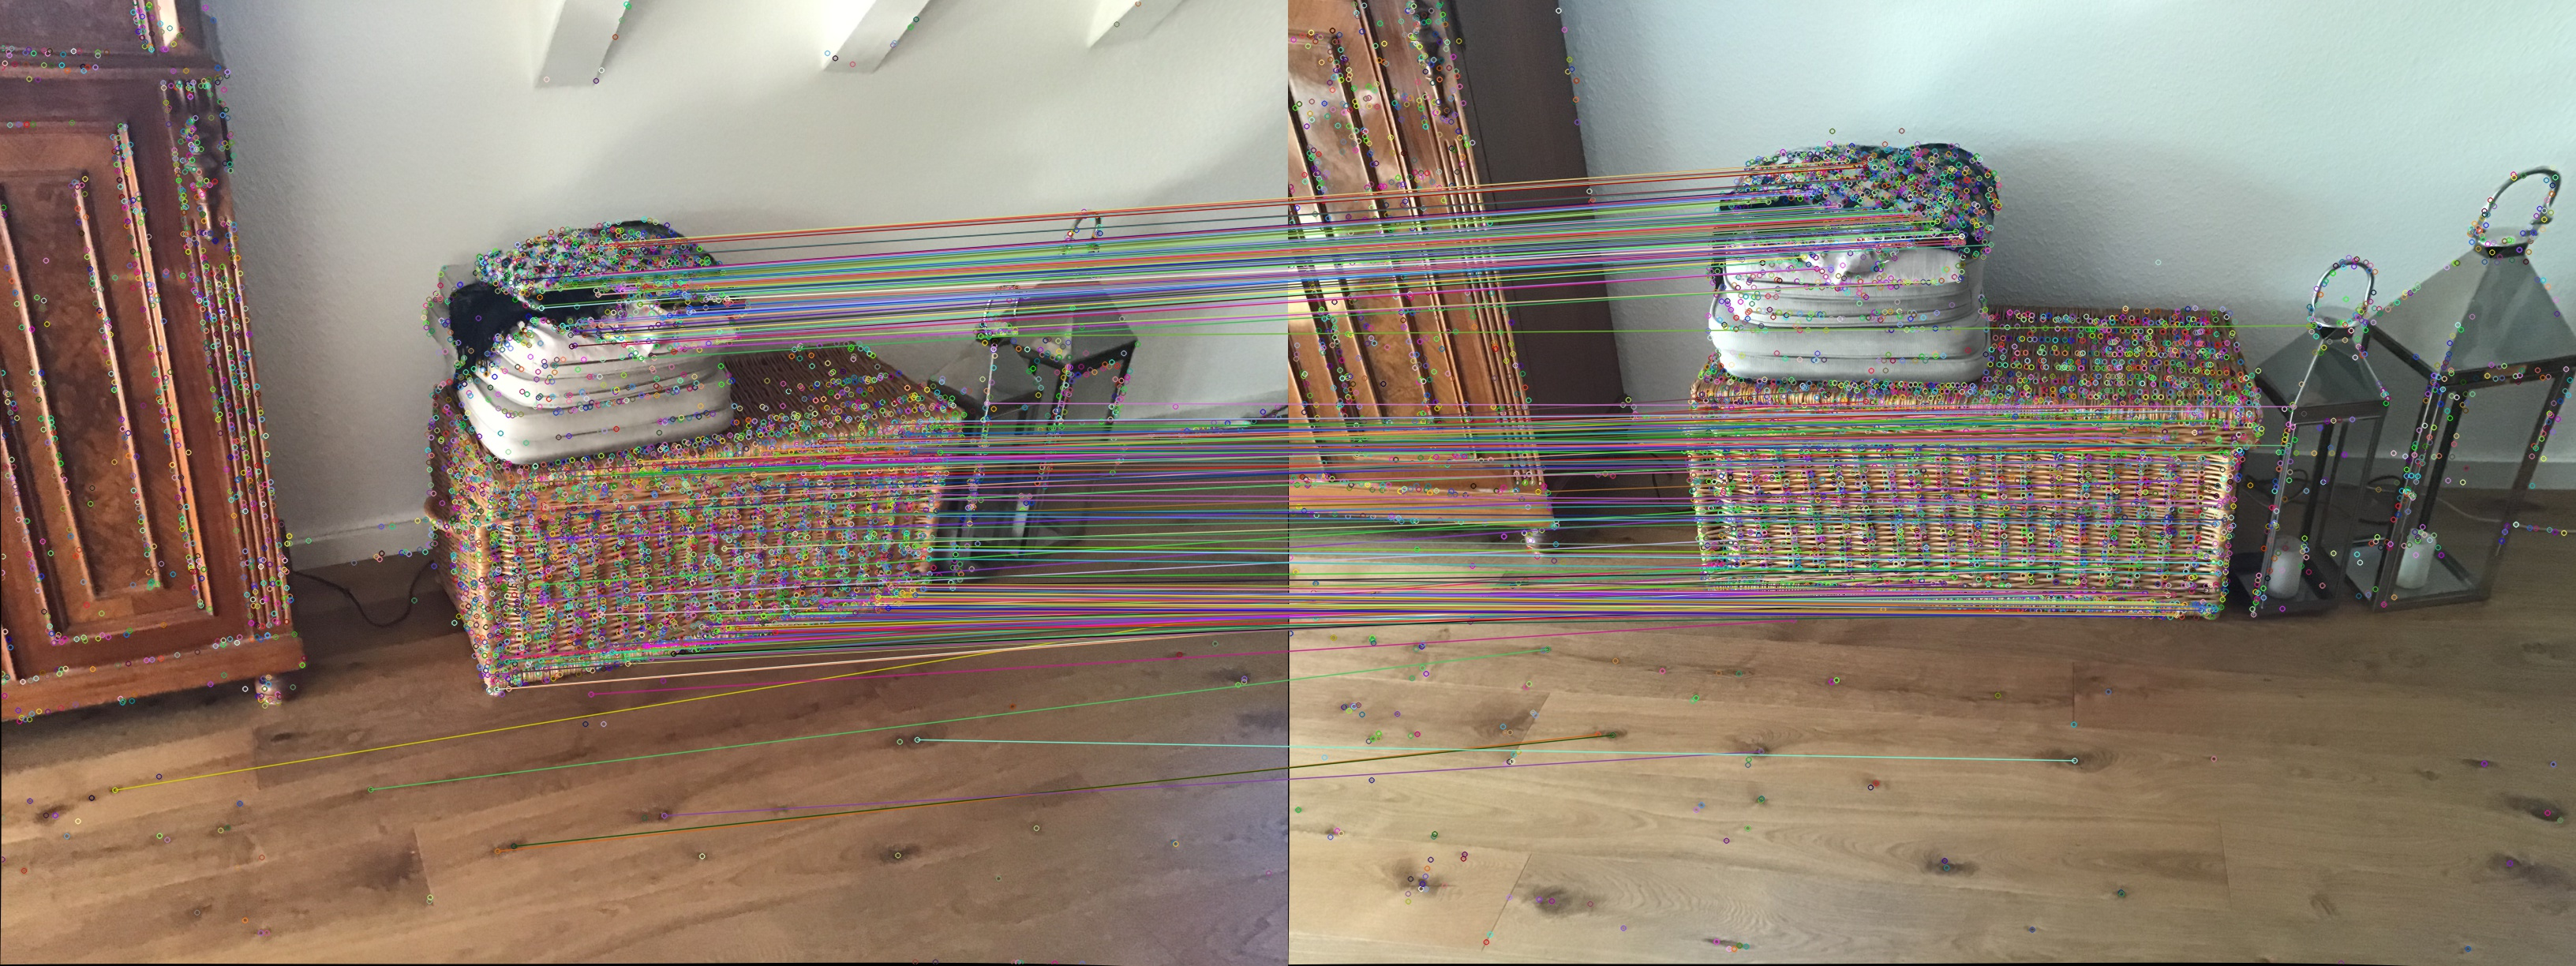
\includegraphics[width=\textwidth]{src/img/box_first_pair_with_matches.jpg}
    \caption{Das erste Bildpaar, mit Matches und Keypoints}
    \label{fig:box-first-pair-with-matches}
\end{figure}

\begin{figure}
    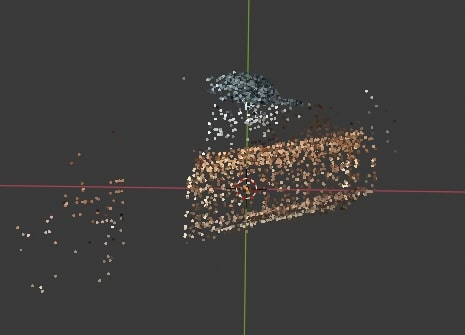
\includegraphics[width=\textwidth]{src/img/box_model.jpg}
    \caption{Die rekonstruierten Punkte aus den Bildern der Box. Das Bild zeigt das Modell ungefähr aus der Position der ersten Kamera.}
    \label{fig:box-model}
\end{figure}

\begin{figure}
    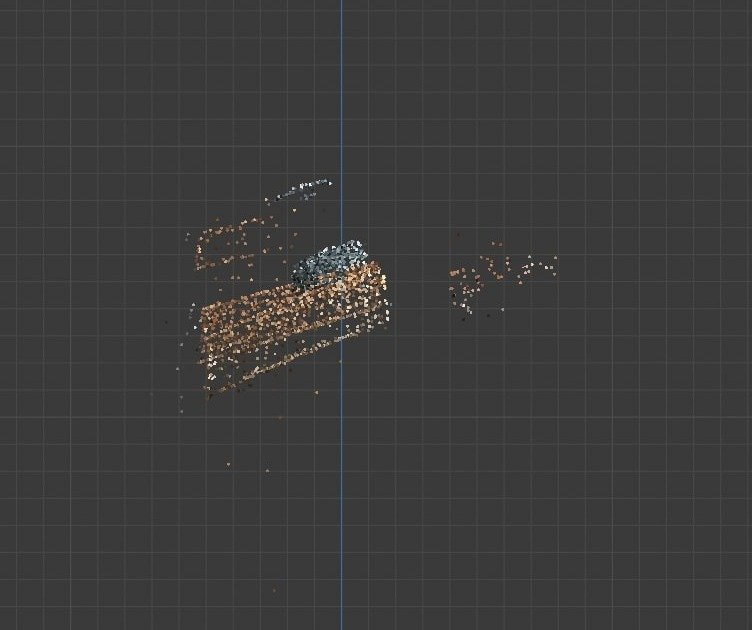
\includegraphics[width=\textwidth]{src/img/box_model_2.jpg}
    \caption{Die rekonstruierten Punkte aus den Bildern der Box. Das Bild zeigt das Modell von der Seite.}
    \label{fig:box-model-2}
\end{figure}
